\label{chapter:correlatos}

\par
\textcolor{red}{Neste capítulo serão apresentados alguns trabalhos relacionados que envolvem mineração de dados...} 

\section{Mineração de Dados Educacionais nos Resultados do ENEM de 2015}

\par
O trabalho de \citeonline{Simon2017} tem como objetivo em gerar um modelo preditivo da base de desempenho médio na área de ciências da natureza e suas tecnologias dos alunos de escolas do ensino médio, baseado nos dados públicos obtidos do Exame Nacional do Ensino Médio (ENEM) de 2015. Tal motivação foi pelo fato do cenário preocupante do baixo desempenho dos alunos do ensino básico no Brasil, conforme os dados de 2015 do PISA (\textit{Programme for International Students Assessment}).

\par
Segundo \citeonline{Simon2017} foi feito o pré-processamento dos dados do ENEM fornecidos pelo INEP, sendo que para cada área avaliada apresentavam-se 25 colunas que representavam uma informação ou variável, onde cada uma delas eram divididas em três categorias: características da escola, indicadores e desempenho. Das 25 variáveis, apenas 9 foram selecionadas como importante para a mineração de dados conforme o indicador da coluna Id representado na Figura 11. 

\begin{figure}[!htp]
	\begin{center}
    \caption{\label{fig:waveform_fig} Variáveis disponibilizadas pelo ENEM por escola.}
	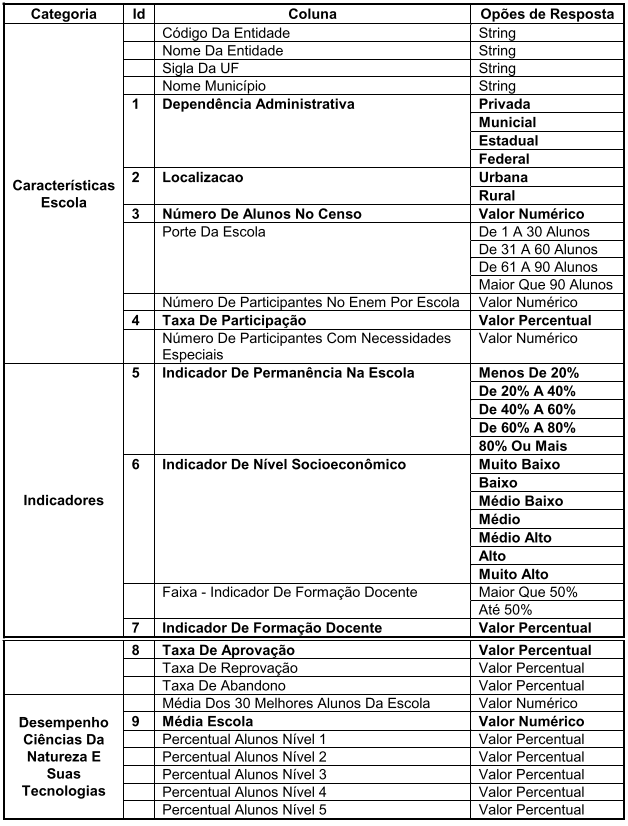
\includegraphics[scale=0.99]{Figuras/Tabela_ENEM.png}
	\end{center}
    \legend{Fonte:\cite{Simon2017}}
\end{figure}

\par
\citeonline{Simon2017} destacaram que a variável Média Escola indicava o desempenho médio dos alunos da escola na área de ciências da natureza e suas tecnologias, onde esses dados eram fornecidos como valor numérico pelo INEP, então para facilitar a mineração dos dados, ele teve que converte-lo para uma categoria mais limitada que foi dividida em quatro valores possíveis, segundo a escala prevista pelo INEP conforme a Figura 12. Os dados fornecido pelo INEP, vinham em uma planilha no formato .xlsx e teve que ser convertido para .csv, pois, o formato não era suportado pelo software WEKA.


\begin{figure}[!htp]
	\begin{center}
    \caption{\label{fig:waveform_fig} Categoria para os valores Média Escola.}
	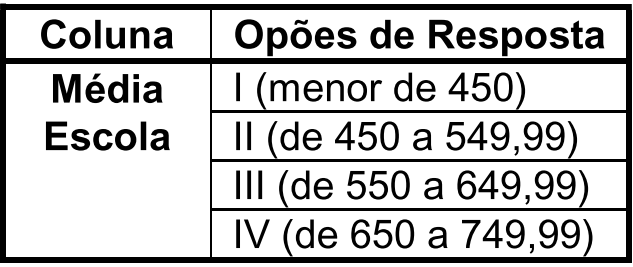
\includegraphics[scale=0.50]{Figuras/Tabela_ENEM_2.png}
	\end{center}
    \legend{Fonte:\cite{Simon2017}}
\end{figure}

\par
Relacionando os fatores socioeconômicos e o índice de desempenho médio em ciências da natureza e sua tecnologias dos alunos, \citeonline{Simon2017} construiu um modelo preditivo utilizando a técnica de mineração de árvore de decisão. Tal técnica, usou o algoritmo j48 através do software WEKA, que foi executado utilizando a opção de \textit{cross-validation}, onde o valor para \textit{fold} era igual a 10 e com a variável depedente Média Escola. Com a árvore obtida, demonstrou como variável independente mais relevante foi a variável Tipo Escola, que se divide entre quatro valores: privada, federal, estadual e municipal.

%Variavel dependete seria o resultado e a variavel independente seria o caminho que ele iria percorre até o resultado. Exemplo: variavel dependete (aluno passou | aluno não passou), variavél independente(entregou os trabalhos, participou das aulas, tirou nota boa na prova, numeros de faltas e etc).

\par
Depois da variável Tipo Escola, a variável hierarquicamente seguinte é a Nível socioeconômico e a partir dela as váriaveis seguintes se alternam de posição conforme as funções dos valores dos níveis superiores. Como resultado, sobre o desempenho médio dos alunos na área de ciências da natureza e suas tecnologias, as categorias que mais se destacaram foram a III e IV, acima de 550 pontos, que ocorreram nas escolas: privadas e estaduais com o nível socioeconômico muito alto, federais com o nível médio alto e muito alto e municipal com o nível médio alto.

\par
\textcolor{red}{Há alguns pontos deste trabalho que se relacionam ao trabalho que pretendo fazer, uma delas é a base de dados dos fatores socioeconômico e outras informações fornecidos do ENEM pelo INEP, que esta relacionado na parte de pré-processamento, é semelhante aos dados fonecidos pela Comissão Permanente do Vestibular (CPV) da UFRR, como base eu poderia pegar as mesmas variáveis que foram escolhidas no trabalho de \citeonline{Simon2017} para agilizar o meu trabalho de minerar os dados mais imporntante para solucionar o meu problema.}
\par
\textcolor{red}{Outro ponto importante é o modelo preditivo que eles abordaram, que é a técnica de mineração de Árvore de Decisão que utiliza o algoritmo J48 do software WEKA, já que eu utilizarei a mesmo conceito de modelo, poderia utilizar a opção de \textit{cross-validation}, no caso o K-\textit{folds}, que ele usou para os treinos e testes dos dados para a validação do modelo.}



\section{Prática de Mineração de Dados no Exame Nacional do Ensino Médio}

\par
O trabalho de \citeonline{Silva2014}, apresenta um estudo de mineração de dados educacionais, mais especificamente, utilizando a tarefa de Associação de Dados de MD no intuito de encontrar padrões de regras nos dados dos questionários socioeconômicos e resultados das provas do Exame Nacional de Ensino Médio (ENEM), fornecidos pelo INEP. O objetivo é de executar as etapas do KDD para o processamento dos dados do ENEM, de modo que por consequência, se utilize a técnica de associação para se encontrar regras proporsicionais que relacionam os fatores socioeconômicos do candidato com o seu desempenho na prova.

\par
Para o trabalho de \citeonline{Silva2014}, foi utilizado o banco de dados com os questionários socioeconômico e os desempenhos da prova do ENEM de 2010, fornecido pelo INEP, onde, para acessar os dados do banco dele, foi usado os softwares Oracle Express Edition 11g e PL/SQL Developer que permitem a extração dos dados que foram determinado para o foco da pesquisa. Os dados utilizados para fazer a mineração de dados, foi da região Sudeste das suas capitaias: Vitória, Belo Horizonte, São Paulo e Rio de Janeiro.

\par
Na parte de pré-processamento, foi selecionado somente os dados das capitais do Sudeste que resultaram em 452.710 alunos, que entretanto, foram eliminados 310.000 alunos das quatros capitais, pois, eles não compareceram no dia da prova. As questões selecionadas para a pesquisa  foram de quantas pessoas moravam com o candidato, a renda familiar mensal, o nível de escolaridade da mãe e o tipo de escola que cursou no ensino médio. Sendo que essas questões foram analisadas para saber se contribuia, interferia ou afetava a nota e o desempenho do candidato na prova.

\par
Baseado nas respostas das questões analisadas, a nota da prova objetiva foi classificada conforme o conceito mostrada na Figura 13. Para a preparação da regra de associação, \citeonline{Silva2014} fez uma limpeza e integração nos dados, alterando as colunas principais para binominais, quer dizer, em 0 e 1, sendo 1 a opção que foi respondida no questionairo e 0 para o restante das opções que não foram escolhida no mesmo questionario, isso aplica tambem a categoria da prova, como podemos ver representado na Figura 14, onde o aluno não foi inserido sendo três de quatro delas. 


\begin{figure}[!htp]
	\begin{center}
    \caption{\label{fig:waveform_fig} Relação de tranformação da nota em conceito.}
	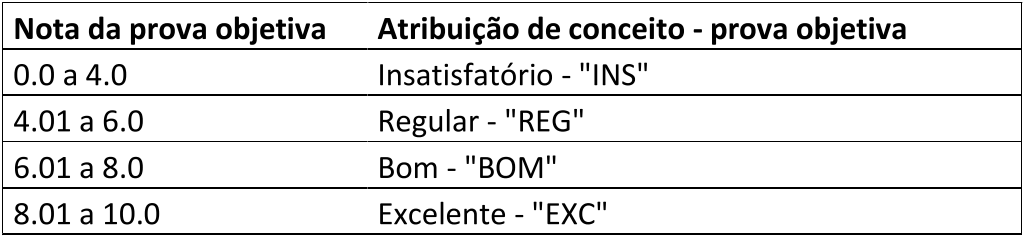
\includegraphics[scale=0.50]{Figuras/Prova_objetiva.png}
	\end{center}
    \legend{Fonte:\cite{Silva2014}}
\end{figure}

\begin{figure}[!htp]
	\begin{center}
    \caption{\label{fig:waveform_fig} Amostragem de alguns dos dados limpos e integrados.}
	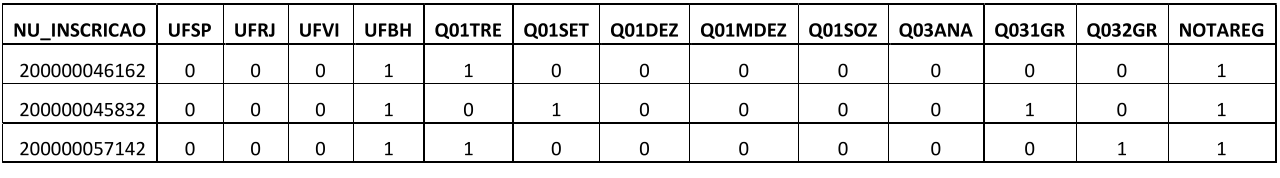
\includegraphics[scale=0.49]{Figuras/Dados_limpos_integrados.png}
	\end{center}
    \legend{Fonte:\cite{Silva2014}}
\end{figure}

\par
Observando a segunda linha da Figura 14, percebemos que o candidato é da cidade de Belo Horizonte, mora no total de sete pessoas contando com ele, a mãe dele possui o 1º grau de nível de escolaridade e que a classificação da nota da prova objetiva dele é regular. Para o melhor entendimento, \citeonline{Silva2014} especifica os critérios das colunas, que são:

\begin{itemize}
    \item \textbf{NU\_INSCRICAO:} O numero de identificação do candidato. 
    \item \textbf{UFXX:} A sigla da cidade onde o candidato mora.
    \item \textbf{QXXABC:} Sendo XX a questão escolhida de acodo com o questionario socioeconômico, ABC representa alternativa escolhida da questão de forma abreviada.
    \item \textbf{NOTAXXX:} Sendo XXX a classificação da nota da prova que o candidato conseguiu. 
\end{itemize}

\par
Para os experimentos que foram feitos, \citeonline{Silva2014} utilizou o software RapidMiner 5.1 que usa o codigo abeto Java, e para a tarefa de associação de dados, é usado o algoritmo A Priori que na etapa de verificação de itens conjuntos ele faz um processo interativo para a combinação de itens. Este algoritmo realiza busca por largura e é definido em três caracteristicas: suporte mínimo, confinaça mínima e K-itemset. Lembrando que o suporte é a frequência o qual uma regra é aplicada em um determinado conjunto de dados e a confiança mede a confiabilidade da interferência feita por uma regra. 

\par
Conforme a Figura 15, \citeonline{Silva2014} observou que a medida que o suporte e a confiança diminuia, o número de regras aumentava.   

\begin{figure}[!htp]
	\begin{center}
    \caption{\label{fig:waveform_fig} Simulação de Suporte e Confiança.}
	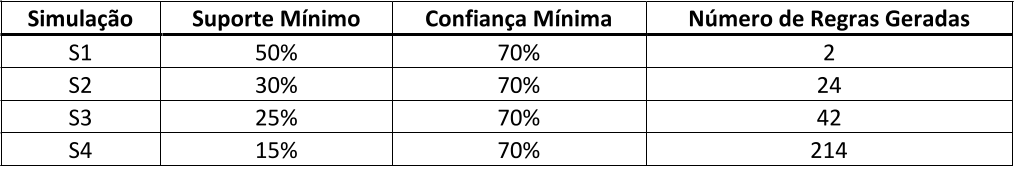
\includegraphics[scale=0.49]{Figuras/Simulacao_suporte_confianca.png}
	\end{center}
    \legend{Fonte:\cite{Silva2014}}
\end{figure}

\par
Das quatros simulações, em cada uma se analisou o seguinte: na simulação 1, a regra aplicada era se o aluno era de ecola publica então a sua nota prova seria regular (76\% de confiança, ocorre 53\% dos alunos) e a outra regra se o aluno tirou nota regular na prova então ele é de escola publica (80\% de confiança, ocorre 53\% dos alunos). Na simulação 2 a primeira regra com confiança mais baixa gerada era se o candidato morasse com quartro e sete pessoas então ele era de escola pública (74\% de confiança, ocorre 31\% dos alunos) e a ultima regra com maior confiança era se os pais tivessem escolaridade de até o primeiro grau então ele era de escola pública (89\% de confiança, ocorre 36\% dos alunos).

\par
Na simulação 3, a primeira regra gerada de menor confiança é se os pais tivessem escolaridade de até o 1º grau então o candidato é de escola pública e a nota da prova é regular (71\% de confiança, ocorre 28\% dos alunos), e a ultima regra com maior confiança e se o candidato é de escola pública e possui pais com escolaridade de até o 1º grau, então sua nota da prova é regular (90\% de confiança, ocorre 19\% dos alunos). Na simulação 4, \citeonline{Silva2014} observou que alguns atributos como escolaridade dos pais e a renda familiar levava o candidato a obter uma nota regular ou vim de uma escola pública, como podemos perceber na ultima regra com maior confiança na Figura 16.

% Podemos evidenciar na penúltima regra que, se o aluno tirou nota regular na prova, os pais tiveram escolaridade até o primeiro grau e a renda da família for de um a três salários mínimos então o aluno estudou em escola pública com 92% de confiança, ocorrendo em 19% dos alunos

\begin{figure}[!htp]
	\begin{center}
    \caption{\label{fig:waveform_fig} Simulação 4, Suporte Mínimo 25\% e Confiança Mínima 70\%.}
	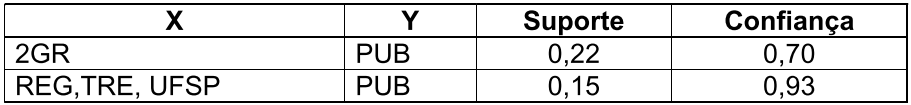
\includegraphics[scale=0.49]{Figuras/Simulacao_quatro.png}
	\end{center}
    \legend{Fonte:\cite{Silva2014}}
\end{figure}

\par
Como representado na Figura 17, \citeonline{Silva2014} verificou que ao diminuir o valor do suporte mínimo, há um acréscimo em casos encontrados na base de dados que utiliza associação de dados, em que se term regras mais verdadeiras, chegando pelo menos a 90\% de confiança, que são geradas na simulação correspondentes. Para a demonstração, \citeonline{Silva2014} criou faixas de confinças que começava a partir de 70\%, onde, cada faixa era verificada entre as simulações com a quantidade de regras que eram geradas, como por exemplo, na simulação 1, dentre as duas regras, se tinha de 76\% e 81\% de confiança, então ele se enquadra na faixa de 70\% até 80\%, totalizando 50\%..

\begin{figure}[!htp]
	\begin{center}
    \caption{\label{fig:waveform_fig} Sintetização das simulações.}
	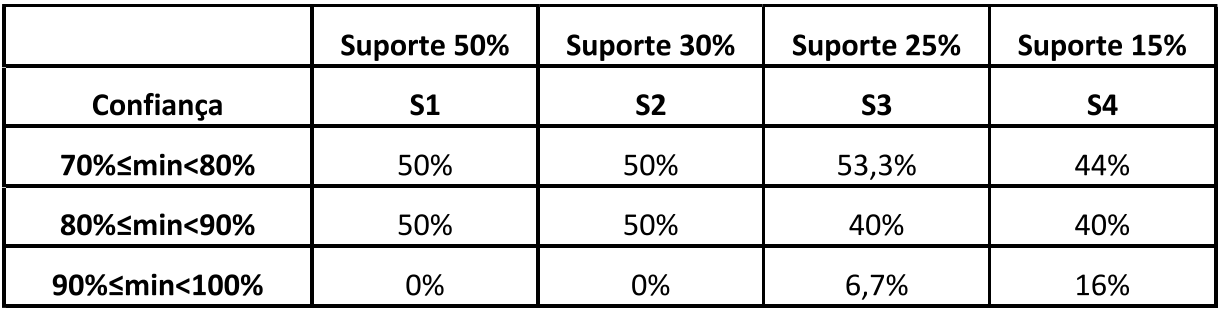
\includegraphics[scale=0.49]{Figuras/Sintetizacao_simulacoes.png}
	\end{center}
    \legend{Fonte:\cite{Silva2014}}
\end{figure}

\par
Contudo, nas regras de maior confinaça obtidos com base nas duas ultimas simulações, \citeonline{Silva2014} verificou que candidatos de São Paulo que moram com quatro a sete pessoas, com renda familiar de até trê salarios mínimos, com pais de escolaridade de até 1º grau e com a nota regular obtida no ENEM, então ele é de escola pública, o que reforça que a educação das escolas públicas das capitais da região sudeste está em um nível baixo. Então \citeonline{Silva2014} conclui que com o conhecimento obtido a partir dos resultados, como alta quantidade de pessoas que moram com o candidato, baixa renda familiar e pais com escolaridade de nível primário, são atributos que afetam o baixo desempenho do candidato. 

\textcolor{red}{No trabalho de \citeonline{Silva2014}, demonstra casos semelhantes que poderar ocorrer no meu tralho, como por exemplo, utilizar dados obtidos do questionario socioeconômico pelo INEP (que no meu caso será pelo CPV), para poder relacionar qual destas questões é um dos motivos que afetam o desempenho do candidato na prova, outro ponto, é a eliminação de ruído de dados na parte de pré-processamento, já que nem todos os candidatos inscritos para o vestibular, por algum motivo, não comparecerão para fazer a prova, então será nescessario tirar os candidatos que não participaram.}

\par
\textcolor{red}{O algoritmo que \citeonline{Silva2014} utilizou para a mineração de dados foi o A Priori, que faz a verificação dos dados através de um processo interativo para combina-los, para então se obter um resultado. Como observado, poderia utilizar como exemplo as técnicas, algoritmo e as questões escolhidas do questionério socioecnômico abordados pelo \citeonline{Silva2014} em conjunto com as outras técnicas e outros conceitos apresentado no meu trabalho, para poder assim, obter mais exatidão e aprimoraramento nos resultados obtidos.}

\par
\textcolor{red}{Um possível problema que eu encontraria se eu fosse basear os exemplos de \citeonline{Silva2014}, é que as questões do questionario socioeconômico fornecidas pelo INEP vem com alternativas de escolha para o candidato responder, o que é diferente das questões fornecido pelo CPV que é resposta direta, um exemplo de uma das questões do questionario socioecômico do ENEM, a questão sobre a quantidade de pessoas que moram com o candidatos, se tem as seguintes alternativas: (a) três pessoas, (b) quatro pessoas, (c) sete pessoas e (d) mais de sete pessoas.}

\section{Descoberta de Conhecimento Sobre o Processo Seletivo da UFPR}

\par
O trabalho de \citeonline{Martinhago2005}, tem como objetivo geral de traçar o perfil dos candidatos ao processo de seleção para a admissão no ensino superior da Universidade Federal do Paraná (UFPR) do campus de Curitiba, utilizando a técnica de mineração de dados Árvore de Decisão através dos algoritmos de classificação J48.J48 e J48.PART, implementados pelo software WEKA. \citeonline{Martinhago2005} utilizou a base de dados dos questionarios socio-educacional realizado durante a inscrição do vestibular feito em 2003, os dados do cadastro geral e os dados das notas obtidas na prova e redação, em conjunto com a nota, média das notas e os status (resultado do vestibula) do candidato pelo ENEM. 

\par
Na fase de Pré-processamento, na parte de seleção de dados, \citeonline{Martinhago2005} juntou os 31 itens do questionario sócio-educacional com os 24 itens do cadastro geral, para formar uma planilha com base de dados de 55 itens (atributos), para servir como base referêcial para aplicação das técnicas de mineração. Ao analisar a base de dados, foi detectado inúmeros itens de dados em branco, valores absusrdos ou erro de digitação, logo, \citeonline{Martinhago2005} teve que prencher esses dados com a letra N (NULL), pois, a ferramenta WEKA que foi utilizado, nescessita que todos os registros estejam preenchidos. Também foi eliminado atributos que eram repetidos por causa da junção das duas planilha e dados que eram irrelevante para a pesquisa, tais como protocolo, bairro, CEP e etc.

\par
Na fase de Mineração de Dados, \citeonline{Martinhago2005} utilizou a ténica de classificação de mineração, a Árvore de decisão, utilizando o algoritmo J48 através do software WEKA, para a criação do modelo preditivo aplicado na base de dados obtidos de 46.532 candidatos. No momento, foram realizado testes onde foi selecionado alguns atributos, tais como, idade, sexo, notas e etc, nos testes seguinte, foi utilizado os mesmos atributos dos testes anteriores em conjunto com alguns atributos culturais e sócio-educacional, tais como, o turno cursado (se fez cursinho ou não), o tipo de escola e etc. Sucessivamente, foram realizados outros testes com outro atributos.

\par
Utilizando o algoritmo J48, em cada execução, varias regras foram geradas e o resultados obtidos para cada base de dados analisados foi o seguinte: para a base de dados dos candidatos ao 11 cursos mais concorridos, \citeonline{Martinhago2005} observou que o conjuntos de notas categorizados com valores acima da faixa de 5 pontos, influênciam na aprovação do candidato, principalmente as notas de redação e língua portuguesa e outras em geral, outra regra relevante, foi de candidatos com notas na faixa de 6 pontos (4,208 a 8,969 pontos) ou acima no ENEM, alcançaram sucesso do vestibular, um exemplo, candidatos para o curso de Direito que obtem nota em Química, Biologia e Matemática acima da faixa de 5 pontos (4,91 a 9,80), segundo \citeonline{Martinhago2005} geralmente tem chance de ser classificado após a análise da redação.

\par
Para o curso mais concorrido, que no caso foi Medicina, segundo \citeonline{Martinhago2005} as notas obtidas nas provas do vestibular e o do ENEM, foi o principal fator que influenciou na aprovação do candidato ao contrário dos fatores sócio-econômico e culturais, que não foram considerados relevantes nos testes realizados, sendo que nas pesquisas do INEP, fatores como renda familiar, escolaridade dos pais, ter feito cursos de pré vestibular e ter estudado em escola particular ou pública, seriam determinates para influenciar a aprovação do candidato no vestibular para o curso de Medicina, porém, mesmo não sendo os principais fatores que influenciam, ainda sim as condições sócio-econômicas interferem na aprovação desse curso. 

\par
Para a base de dados dos candidatos aos onze cursos menos concorridos, através das regras geradas nos testes, segundo \citeonline{Martinhago2005} a notas que influênciaram na aprovação dos candidatos foi em Geografia, Redação, Língua Estrangeira e História e as notas que não foram importantes para aprovação eram Matemática, Química e Física. \citeonline{Martinhago2005} percebeu que uma das regras mais importante como a escolaridade dos pais, influênciavam na aprovação. Alguns dos fatores interessantes que foram extraídos é de que nos cursos menos concorridos os candadatos que foram aprovados, tinham concluído o Ensino Médio a mais de 5 anos e que vinham de escolas públicas ao contrário dos cursos mais concorridos onde essa relação não era frequente, outro fator, é de o candidato ter ou não feito cursinho, não influenciava no resultado.

\par
Para a base de dados contendo os dados de todos os candidatos ao vestibular, \citeonline{Martinhago2005} notou que para as regras geradas, a maioria dos candidatos moram com os pais, não trabalham e que estão em uma faixa de 17 a 20 anos. Observou também, que as pontuações obtidas pelos candidatos para um curso onde na área dele a nota de algumas disciplinas são essênciais para o vestibular, não tem tanta influência no resultado como a pontuação obtida em outras disciplinas de outras áreas, por exemplo na área de exatas, como o curso de Estatística onde as notas de Geografia, Língua estrangeira e História influenciam na aprovação do candidato, ao contrário da área de humanas como Ciências Sociais, onde notas como Matemática, Física e Química, influenciam nos resultados de aprovação. 

\textcolor{red}{Assim como os trabalhos anteriores que são semelhantes ao que eu proponho, o trabalho de \citeonline{Martinhago2005} usa como base de dados para o seus experimentos os dados dos questionários sócioeconômico e os dados do cadastro geral dos candidatos do vestibular da UFPR para o seus testes de mineração, a diferença é que \citeonline{Martinhago2005} fez junção com alguns dados forncecidos pelo ENEM para produzir mais regras e ter um melhor resultado na sua predição. Outro fator semelhante é que é utilizado a técnica de mineração a Árvore de Decisão usando o algoritmo J48 pela ferramenta WEKA para a geração de regras para se obter os resultados. Assim como \citeonline{Martinhago2005} encontrou alguns dados em branco e atributos repetidos e teve que adaptar para o software WEKA, presumo que encontrarei o mesmo problema durante a seleção e pré-processamento de dados.}

%==========================================================
% REVISÃO SISTEMÁTICA
%==========================================================
\section{Síntese dos Trabalhos Correlatos}

\par
\textcolor{red}{Foram analisados na literatura, trabalhos que discorrem sobre a utilização de mineração de dados em uma base de dados de um vestibular, para a criação de um modelo preditivo através de regras criadas, a fim de gerar perfis dos candidatos que são aprovados ou saber quais foram os fatores que afetaram ou contribuiram no desempenho do candidato na sua nota da prova.} 

\par
\textcolor{red}{Em \cite{Simon2017}, motivados pelos problemas de infraestrutura apresentados pelo Censo Escolar da Educação Básica de 2016, criaram um modelo preditivo que relacionava o perfil socioeconômico dos candidatos fornecidos pelo INEP com a infraestrutura das escolas apresentados pelo PISA para associar ao desempenho dos alunos em exames, no caso, a prova do ENEM.}

\par
\textcolor{red}{\citeonline{Silva2014}, em suas pesquisas identificaram fatores que diminuem o desempenho dos candidatos, através da técnica de mineração baseada em regras de associação que utilizavam diferentes parametrizações do algoritmo A Priori. Dados esses utilizados dos questionários socioeconômicos preenchidos pelos candidatos nas edição de 2010 do ENEM da região Sudeste. Essas informações, especificamente as respostas de quatro perguntas, são relacionadas com o resultado de desempenho desses alunos.}

\par
\textcolor{red}{Por fim, \citeonline{Martinhago2005} investigou a base de dados sobre os vestibulandos da UFPR de 2003, como os dados dos questionários socioeconômico preenchidos pelos candidatos durante as inscrições, os dados do cadastro geral que contém as notas obtidas da prova e redação e o resultado do vestibualar em conjunto com as notas e média das notas obtidas pelo ENEM, para poder traçar o perfil dos vestibulandos, utilizando a técnica de mineção Árvore de Decisão.}

\par
\textcolor{red}{A Tabela X visa prestar uma breve comparação entre as características chaves dos trabalhos relacionados e as propostas deste trabalho.}

\par
\textcolor{red}{Seleção de dados importantes para a base de dados, Eliminação de ruídos e atributos repetidos na base de dados, Transformação dos dados em formato apropriado para mineração, Mineração de dados para extraír informações importantes, Identificação do conhecimento extraído na busca de padrões, Resultados da solução de um possivel problema.}




%==========================================================
%PLANEJAMENTO DA REVISÃO SISTEMÁTICA
%==========================================================
\subsection{Planejamento da Revisão Sistemática}
\textbf{Objetivo:} Este estudo tem o objetivo esquematizado a partir da estrutura do paradigma GQM (do ingles \textit{Goal,Question and Metric})\cite{basili1994experience}.

\begin{table}[h!]
\centering
\label{}
\begin{tabularx}{\textwidth}{|l|X|}
\hline
Analisar & Publicações científicas através de um estudo baseado em revisão sistemática \\ \hline
Com propósito de & Identifica-las \\ \hline
Com relação as & Vantagens e desvantagens da utilização de assertiva e transformações de código na verificação do código na linguagem de descrição VHDL \\ \hline
Do ponto de vista do & Pesquisador \\ \hline
No contexto & Acadêmico ou industrial para verificação de assertivas na linguagem de descrição VHDL \\ \hline
\end{tabularx}
\caption{Objetivo do estudo utilizando o paradigma GQM}
\end{table}

\textbf{Formulação da Pergunta:} Buscamos respostas para as seguintes perguntas:
\begin{itemize}
\item \textbf{Q1:} Quais são os métodos para verificação de circuitos lógicos descritos na linguagem de programação VHDL?
	\begin{itemize}
	\item \textbf{Q1.1:} Foi desenvolvido e está disponível alguma ferramenta para aplicação do método?
	\item \textbf{Q1.2:} Qual a técnica de exploração de estados para circuitos lógicos?
	\item \textbf{Q1.3:} O método proposto é baseado em técnicas de verificação de software?
	\item \textbf{Q1.4:} Como o método proposto valida pré e pós condições no programa?
	\item \textbf{Q1.3:} Foi utilizado algum \textit{benchmark} de programas em VHDL para experimentação e o mesmo encontra-se disponível?
	\item \textbf{Q1.4:} Quais as perspectivas futuras para melhorar da aplicação do método proposto?
	\end{itemize}
\end{itemize}

